% Options for packages loaded elsewhere
\PassOptionsToPackage{unicode}{hyperref}
\PassOptionsToPackage{hyphens}{url}
%
\documentclass[
  12pt,
]{article}
\usepackage{amsmath,amssymb}
\usepackage{lmodern}
\usepackage{ifxetex,ifluatex}
\ifnum 0\ifxetex 1\fi\ifluatex 1\fi=0 % if pdftex
  \usepackage[T1]{fontenc}
  \usepackage[utf8]{inputenc}
  \usepackage{textcomp} % provide euro and other symbols
\else % if luatex or xetex
  \usepackage{unicode-math}
  \defaultfontfeatures{Scale=MatchLowercase}
  \defaultfontfeatures[\rmfamily]{Ligatures=TeX,Scale=1}
\fi
% Use upquote if available, for straight quotes in verbatim environments
\IfFileExists{upquote.sty}{\usepackage{upquote}}{}
\IfFileExists{microtype.sty}{% use microtype if available
  \usepackage[]{microtype}
  \UseMicrotypeSet[protrusion]{basicmath} % disable protrusion for tt fonts
}{}
\makeatletter
\@ifundefined{KOMAClassName}{% if non-KOMA class
  \IfFileExists{parskip.sty}{%
    \usepackage{parskip}
  }{% else
    \setlength{\parindent}{0pt}
    \setlength{\parskip}{6pt plus 2pt minus 1pt}}
}{% if KOMA class
  \KOMAoptions{parskip=half}}
\makeatother
\usepackage{xcolor}
\IfFileExists{xurl.sty}{\usepackage{xurl}}{} % add URL line breaks if available
\IfFileExists{bookmark.sty}{\usepackage{bookmark}}{\usepackage{hyperref}}
\hypersetup{
  pdftitle={There Votes the Neighborhood: Gentrification, Displacement, and Political Participation in Atlanta},
  pdfauthor={Kevin Morris},
  hidelinks,
  pdfcreator={LaTeX via pandoc}}
\urlstyle{same} % disable monospaced font for URLs
\usepackage[margin=1in]{geometry}
\usepackage{longtable,booktabs,array}
\usepackage{calc} % for calculating minipage widths
% Correct order of tables after \paragraph or \subparagraph
\usepackage{etoolbox}
\makeatletter
\patchcmd\longtable{\par}{\if@noskipsec\mbox{}\fi\par}{}{}
\makeatother
% Allow footnotes in longtable head/foot
\IfFileExists{footnotehyper.sty}{\usepackage{footnotehyper}}{\usepackage{footnote}}
\makesavenoteenv{longtable}
\usepackage{graphicx}
\makeatletter
\def\maxwidth{\ifdim\Gin@nat@width>\linewidth\linewidth\else\Gin@nat@width\fi}
\def\maxheight{\ifdim\Gin@nat@height>\textheight\textheight\else\Gin@nat@height\fi}
\makeatother
% Scale images if necessary, so that they will not overflow the page
% margins by default, and it is still possible to overwrite the defaults
% using explicit options in \includegraphics[width, height, ...]{}
\setkeys{Gin}{width=\maxwidth,height=\maxheight,keepaspectratio}
% Set default figure placement to htbp
\makeatletter
\def\fps@figure{htbp}
\makeatother
\setlength{\emergencystretch}{3em} % prevent overfull lines
\providecommand{\tightlist}{%
  \setlength{\itemsep}{0pt}\setlength{\parskip}{0pt}}
\setcounter{secnumdepth}{5}
\usepackage{rotating}
\usepackage{setspace}
\newcommand{\beginsupplement}{\setcounter{table}{0}  \renewcommand{\thetable}{A\arabic{table}} \setcounter{figure}{0} \renewcommand{\thefigure}{A\arabic{figure}}}
\usepackage{lineno}
\usepackage{booktabs}
\usepackage{longtable}
\usepackage{array}
\usepackage{multirow}
\usepackage{wrapfig}
\usepackage{float}
\usepackage{colortbl}
\usepackage{pdflscape}
\usepackage{tabu}
\usepackage{threeparttable}
\usepackage{threeparttablex}
\usepackage[normalem]{ulem}
\usepackage{makecell}
\usepackage{xcolor}
\ifluatex
  \usepackage{selnolig}  % disable illegal ligatures
\fi
\newlength{\cslhangindent}
\setlength{\cslhangindent}{1.5em}
\newlength{\csllabelwidth}
\setlength{\csllabelwidth}{3em}
\newenvironment{CSLReferences}[2] % #1 hanging-ident, #2 entry spacing
 {% don't indent paragraphs
  \setlength{\parindent}{0pt}
  % turn on hanging indent if param 1 is 1
  \ifodd #1 \everypar{\setlength{\hangindent}{\cslhangindent}}\ignorespaces\fi
  % set entry spacing
  \ifnum #2 > 0
  \setlength{\parskip}{#2\baselineskip}
  \fi
 }%
 {}
\usepackage{calc}
\newcommand{\CSLBlock}[1]{#1\hfill\break}
\newcommand{\CSLLeftMargin}[1]{\parbox[t]{\csllabelwidth}{#1}}
\newcommand{\CSLRightInline}[1]{\parbox[t]{\linewidth - \csllabelwidth}{#1}\break}
\newcommand{\CSLIndent}[1]{\hspace{\cslhangindent}#1}

\title{There Votes the Neighborhood: Gentrification, Displacement, and Political Participation in Atlanta}
\author{Kevin Morris\footnote{PhD Student, CUNY Graduate Center, Department of Sociology (\href{mailto:kmorris@gradcenter.cuny.edu}{\nolinkurl{kmorris@gradcenter.cuny.edu}})}}
\date{March 28, 2022}

\begin{document}
\maketitle
\begin{abstract}
TKTKTK
\end{abstract}

\pagenumbering{gobble}
\pagebreak

\pagenumbering{arabic}
\doublespacing

\hypertarget{introduction}{%
\section{Introduction}\label{introduction}}

``And here we are, seniors'' Miss Bertha Darden challenged former mayor and then-mayoral candidate Kasim Reed at a forum on October 22, 2021. ``Where are we going to live? Where are we going to stay?'' The video went viral, attracting tens of thousands of views over the space of a few short days (\protect\hyperlink{ref-McCaffrey2021}{McCaffrey 2021}).

Miss Darden has a long history of confronting the Atlanta city government, and has been active in the fight against gentrification in the city since at least 2012, when her home---along with those of many of her neighbors---in the Peoplestown section of the city faced massive flooding. Following the disaster, the city offered buy-outs to many of the residents, with civil engineering plans for a retention pond and park to prevent future flooding. Miss Darden and her husband, along with three other families, refused the buyouts. Although the Dardens say that Mayor Reed personally assured them they would not have to leave, they were met with a city government willing to use eminent domain to remove these families from their homes. The move was contested in court by the residents, and the legal battle was still ongoing as Reed sought re-election for a nonconsecutive mayoral term (\protect\hyperlink{ref-McCaffrey2021}{McCaffrey 2021}).

Despite the city's stated intention to use the rentention pond and park as anti-flooding measures to protect residents, Miss Darden and others see a clear ulterior motive: a wholesale removal of current residents to make way for wealthier, whiter newcomers. As \protect\hyperlink{ref-Ashly2020}{Ashly} (\protect\hyperlink{ref-Ashly2020}{2020}) explains, these fears may not be unfounded: " neighbourhoods around {[}Peoplestown{]} have transformed over the last decade and a half; each following the same trend: Black and low-income residents pushed out while wealthier and mostly white residents replaced them." Indeed, the Dardens' home Census tract has gone from 86\% Black and just 10\% white in 2009 to 70\% Black and 20\% white in 2020 (ACS 5-Year Estimates).

While the experience of the Dardens and their neighbors presents perhaps an extreme example, it is part of a larger trend in local municipalities investing in public goods without attending to housing stability. Looking at a particular form of investment, a report from the Federal Reserve of San Francisco describes the phenomenon: ``{[}T{]}here is a significant body of literature on the impact of transit on property values, which is intimately tied to the social status of the people who live there'' (\protect\hyperlink{ref-Zuk2015}{Zuk et al. 2015, 18}). Although the process can happen unintentionally, expectations about economic upgrading are central to many public improvement projects. Tax increment financing, or TIF, explicitly assumes that a public investment will result in higher property values, and uses the ensuing expected increase in property taxes as collateral to secure financing for the project (\protect\hyperlink{ref-Weber2002}{Weber 2002}).

This project asks if and how the state-led nature of neighborhood ``upgrading'' and gentrification is translated into local political action. Qualitative scholars have identified how local communities can resist gentrification and displacement, placing these struggles into the broader context of social movement research (e.g., \protect\hyperlink{ref-Betancur2002}{Betancur 2002}). While it seems clear that gentrification can provoke \emph{some} residents into political movement, less is known about how such an experience operates over the full population of residents subject to the pressures of gentrification. Do families facing rising housing costs tune in to local politics at higher rates? Does the experience of leaving a neighborhood behind that was increasingly unaffordable undermine ties to local democracy---or does it anger citizens into participating? Understanding whether citizens turn to the ballot box to contest aggressive state (in)action that allows for gentrification is of signal importance given the austerity turn characteristic of American municipalities following the fiscal crisis at the century's open (\protect\hyperlink{ref-Theodore2020}{Theodore 2020}).

I leverage unique administrative data spanning the course of a decade (2010--2020) that records the home address and electoral turnout of all registered voters. These records are linked across time by unique voter identification numbers, allowing me to track whether and where voters moved between 2010 and 2020. Using a genetic matching algorithm (\protect\hyperlink{ref-Sekhon2011}{Sekhon 2011}) I construct pairs of voters in which one voter lived in 2010 in a neighborhood that went on to gentrify---the ``treated'' voters---while the control voter lived in a 2010 neighborhood that was substantially similar in 2010 but did not go on to gentrify. I then use difference-in-differences / two-way fixed effects models to ask whether those who remained in gentrified neighborhoods participated at different rates than those who stayed in non-gentrified neighborhoods, and whether leaving a gentrified neighborhood influenced turnout differently than leaving a non-gentrified one.

My results paint a surprising picture: for most groups, the experience of living in 2010 in a neighborhood that would go on to gentrify did not influence political participation, whether the voter left their neighborhood or remained in place. Indeed, with the exception of white voters who did not move, my models return fairly precise null estimates, implying that the average Black voter in Atlanta maybe does not incorporate their experience with gentrification into their baseline local political participation---or, at least not in the ballot box.

\hypertarget{gentrification-as-a-state-practice}{%
\section{Gentrification as a State Practice}\label{gentrification-as-a-state-practice}}

The latter half of the 20th century for the American metropolis was characterized by urban flight, disinvestment, and hyper-segregation. In the aftermath of the 1965 civil rights movement, many white Americans fled urban areas, both leading and following jobs out of these areas (\protect\hyperlink{ref-Jackson1985}{Jackson 1985}; \protect\hyperlink{ref-Sugrue1998}{Sugrue 1998}). While middle class white Americans were able to decamp for suburban areas, even relatively wealthy Black Americans were forced to remain in decaying urban neighborhoods thanks to racial steering from the real estate industry and racist lending practices by financial institutions (\protect\hyperlink{ref-Rothstein2017}{Rothstein 2017}). \protect\hyperlink{ref-Massey2003}{Massey and Denton} (\protect\hyperlink{ref-Massey2003}{2003}) documents many of the implications of this \emph{de facto} segregation, demonstrating the vulnerability of Black Americans---regardless of class---to economic adversity. As \protect\hyperlink{ref-Taylor2019}{Taylor} (\protect\hyperlink{ref-Taylor2019}{2019}) shows, the consequences of these restrictive lending practices did more than simply keep Black Americans out of the suburbs: they also inhibited Black residents from buying property in their neighborhoods or investing in property that they did own. Declining tax bases and waning political capital meant that public services in urban areas deteriorated quickly, hastening the out migration of those who could do so (see, for instance, \protect\hyperlink{ref-Phillips-Fein2017}{Phillips-Fein 2017}).

In the late 20th and early 21st centuries, these patterns reversed as Americans began moving back to some urban areas. Increased capital investments (\protect\hyperlink{ref-Birch2009}{Birch 2009}) formed an important part of this back-to-the-city movement (\protect\hyperlink{ref-Hyra2015}{Hyra 2015}). As increasing numbers of highly-educated and highly-compensated Americans sought to live in cities such as San Francisco and New York, communities that had been marginalized (both economically and physically) for a generation or more found themselves residing in areas with increasing potential value. As Samuel Stein argues in \emph{Capital City} (\protect\hyperlink{ref-Stein2019}{2019}), financial capitalists recognized the mismatch between the current and potential income being produced in urban neighborhoods. He explains: ``Real estate speculators choose to invest in a particular location because they identify a gap between the rents that land currently offers and the potential future rents it might command if some action were taken'' (\protect\hyperlink{ref-Stein2019}{Stein 2019, 49}). Stein argues, however, that gentrification is at heart a political issue; it cannot transpire without the state clearing the way for investors to exploit that value gap. Smith (\protect\hyperlink{ref-Smith2002}{2002, 441}, emphasis added) makes this point even more explicitly: ``By the end of the twentieth century,'' he writes, ``gentrification \emph{fueled by a concerted and systematic partnership of public planning with public and private capital} had moved into the vacuum left by the end of liberal urban policy.''

This analysis of the state-led nature of gentrification is echoed in the popular press, where journalists often draw links between state action and increased rents. When discussing the rezoning of the Inwood neighborhood in Manhattan, for instance, the \emph{New York Times} wrote that ``After the rezoning plan was announced in 2013, years before it was enacted, real estate investors swooped into Inwood and bought more than \$610 million in properties'' (\protect\hyperlink{ref-Haag2019}{Haag 2019}). Public infrastructure programs, such as the BeltLine Park in Atlanta, are also led by the state and feared by residents for their potentially displacing effect (\protect\hyperlink{ref-Lartey2018}{Lartey 2018}). Whether the state is explicitly subsidizing development in an area by providing improved public goods or implicitly subsidizing it by allowing for higher-intensity development, the state's involvement is clear. It is perhaps unsurprising, then, that many communities where state investment has historically been virtually nonexistent are fighting back against plans that would increase financial investment in their neighborhoods (e.g. \protect\hyperlink{ref-Lees2018}{Lees, Annunziata, and Rivas-Alonso 2018}).

The state, then, is inherently involved in the gentrification of American cities. State (in)action led to under-investment in these neighborhoods in the 20th century, and state action is now paving the way for private interests to capitalize on that history. And yet, the existing work on gentrification has largely ignored how---or whether---residents hold the state accountable for their changed life circumstances. Scholars have instead focused on the non-state consequences of gentrification, asking questions primarily about whether gentrification leads to displacement (\protect\hyperlink{ref-Hwang2020}{Hwang and Ding 2020}), how it effects education (\protect\hyperlink{ref-Keels2013}{Keels, Burdick--Will, and Keene 2013}), whether it increases employment (\protect\hyperlink{ref-Meltzer2017}{Meltzer and Ghorbani 2017}), its effects on crime (\protect\hyperlink{ref-Papachristos2011}{Papachristos et al. 2011}), and other matters. While these questions certainly have merit, understanding whether residents turn to the ballot to contest gentrification is of key importance given the role of the state in its mechanics.

\hypertarget{the-potentially-politicizing-nature-of-gentrification}{%
\section{The Potentially Politicizing Nature of Gentrification}\label{the-potentially-politicizing-nature-of-gentrification}}

\hypertarget{policy-threat}{%
\subsection{Policy Threat}\label{policy-threat}}

A growing body of literature in political science and sociology documents how citizens respond when they face threatening circumstances. While sociologists have historically focused on ``extra-institutional'' political behavior such as protest and social movement participation, political scientists have often focused more narrowly on political \emph{outcomes} (\protect\hyperlink{ref-Barrie2021}{Barrie 2021}). Both disciplines, however, provide insights into how political behavior is shaped by government action.

Throughout this literature runs the notion of governmental or policy threat: namely, when individuals feel that they or a group to which they belong are being targeted by government policy, they can be mobilized to take action (\protect\hyperlink{ref-TamCho2006a}{Tam Cho, Gimpel, and Wu 2006}). Van Stekelenburg and Klandermans (\protect\hyperlink{ref-vanStekelenburg2013}{2013, 897}) explain: ``The more people feel that interests of the group and/or principles that the group values are threatened, the angrier they are and the more they are prepared to take part in protest to protect their interests and principles and/or to express their anger.'' \protect\hyperlink{ref-Almeida2018}{Almeida} (\protect\hyperlink{ref-Almeida2018}{2018}) characterizes these threats from the state as ``rights eroding'' threats, noting that threats to abortion and welfare programs often spur citizens to take action. \protect\hyperlink{ref-Reese2011}{Reese} (\protect\hyperlink{ref-Reese2011}{2011}) similarly documents how citizens faced with President Bill Clinton's Personal Responsibility and Work Opportunity Reconciliation Act of 1996, which threatened to radically undermine the U.S.'s social safety net, were mobilized into resistance. Key to this mobilization is the understanding that group-level processes are at work: \protect\hyperlink{ref-Piven1979}{Piven and Cloward} (\protect\hyperlink{ref-Piven1979}{1979}) and \protect\hyperlink{ref-Schlozman1979}{Schlozman and Verba} (\protect\hyperlink{ref-Schlozman1979}{1979}), for instance, document how workers become politically engaged when they understand their unemployment as a widespread phenomenon that demands collective government response and not an individual failure.

\protect\hyperlink{ref-Zepeda-Millan2016}{Zepeda-Millán} (\protect\hyperlink{ref-Zepeda-Millan2016}{2016}) offers key insight into how even ``unconventional'' political actors can be mobilized to participate under certain circumstances. He uses the case of Latinos in Fort Myers, Florida, to demonstrate these processes. In 2006, Americans across the country took to the streets to protest \emph{The Border Protection, Antiterrorism, and Illegal Immigration Control Act of 2005} (H.R. 4437), widely considered to be discriminatory toward Latinos. The bill sought to change the penalty for being an undocumented immigrant from a misdemeanor to a felony, and to provide vast new resources for border enforcement. Zepeda-Millán (\protect\hyperlink{ref-Zepeda-Millan2016}{2016, 270}) shows how neighborhood context and the cultivation of shared Latino identities led ``unconventional political actors---from local soccer league players and nannies to farmworkers and ethnic entrepreneurs---to utilize pre-existing neighborhood assets for the purpose of immigrant mass mobilization.''

These policy threats have also been shown to induce citizens to cast ballots at higher rates. Ariel \protect\hyperlink{ref-White2016}{White} (\protect\hyperlink{ref-White2016}{2016}), for instance, documents how strict immigration enforcement led to higher turnout rates among Latinos in counties across the country. Similarly, \protect\hyperlink{ref-Towler2018}{Towler and Parker} (\protect\hyperlink{ref-Towler2018}{2018}) argues that Black Americans turned out at high rates in the 2016 president because of the threat posed to their community by Donald Trump. Tam Cho and colleagues (\protect\hyperlink{ref-TamCho2006a}{2006, 978}), in a study demonstrating higher turnout among Arab Americans who feel threatened, sum up: ``A solid body of evidence\ldots{} indicates that political mobilization is a direct response to the degree of threat and discrimination a group experiences.''

Gentrification can be understood through this same lens; as discussed above, the state plays a central role in the facilitation of gentrification. Although \protect\hyperlink{ref-Thorpe2021}{Thorpe} (\protect\hyperlink{ref-Thorpe2021}{2021}) argues that scholars have not historically acknowledged the importance of law and policy in the easing of gentrification, the scholars and activists have long written about gentrification using the language of rights. Since Henri Lefebvre's 1968 \emph{Le Droit à la Ville} (\protect\hyperlink{ref-Lefebvre1968}{1968}), scholars and activists have counterposed the demands of capital with citizens' ``right to the city'' and, more recently, ``right to stay put'' (see, for instance, \protect\hyperlink{ref-Hartman2002}{Hartman 2002}). Insofar as residents understand gentrification as an infringements on their \emph{right} to their home or community, it likely activates many of the same responses that have been identified in other contexts of policy threat. Given the highly racialized nature of contemporary gentrification (\protect\hyperlink{ref-Freeman2015}{Freeman and Cai 2015}), nonwhite residents may further feel targeted due to the racial identities of their communities.

\protect\hyperlink{ref-Betancur2002}{Betancur} (\protect\hyperlink{ref-Betancur2002}{2002}) explores how these processes play out in the context of West Town (a collection of neighborhoods in Chicago) in the early 1990s and 2000. Betancur notes that, ``Concerned about improving the tax base, city hall did all it could to promote gentrification.'' Ultimately, ``A crucial element at work in West Town was public-sector support for the processes and institutions that made use of public powers of social control to make life miserable for minority low-income residents'' (806). Betancur argues that the state's role in gentrification was contested politically through both institutional and non-institutional means. Gentrification was a major issue in alderman elections in 1999, following the splitting of the area into 4 wards in the aftermath of the 1989 census. But Betancur also shows how the political process played out in non-institutional spaces as well. To take one example, ``Puerto Ricans made great advances in controlling local schools, getting local institutions (e.g., hospitals and churches) to pay attention to their needs and cultural and economic realities, promoting community identity and pride, and gaining respect from political forces'' (802).

Similarly, \protect\hyperlink{ref-Martin2007a}{Martin} (\protect\hyperlink{ref-Martin2007a}{2007}) shows how communities in Atlanta, Georgia, resist political displacement in the face of gentrification. Worried about the rising numbers of newcomers to their neighborhoods, long-term residents created or invested in organizations to represent their interests. Martin describes how new and existing residents of the Belleview neighborhood struggled for the upper political hand: ``For seven years, long-time residents and new residents engaged each other in a series of bitter conflicts over political influence. Through separate organizations, they challenged each other about new neighborhood amenities such as a neighborhood library, a grocery store, and streetscaping in the neighborhood business district. They also sparred over valid means to control crime in the neighborhood, over appropriate neighborhood leadership, and even over the process of gentrification itself'' (616). It is clear that, at least under certain circumstances, long-term residents in gentrifying neighborhoods are able to organize politically---in an electoral sense or otherwise---to contest the gentrification process.

\hypertarget{social-cohesion}{%
\subsection{Social Cohesion}\label{social-cohesion}}

While the policy threat literature indicates that gentrification might lead to \emph{higher} turnout as a community feels itself threatened by the state and by real estate capital, other work indicates that gentrification could \emph{reduce} turnout by undermining social solidarity within a neighborhood. In fact, the lone paper of which I am aware exploring the turnout effects of gentrification (\protect\hyperlink{ref-Knotts2006}{Knotts and Haspel 2006}) comes to this conclusion, finding that turnout for long-term residents in gentrified neighborhoods in Atlanta was lower than long-term residents residing elsewhere. However, because they use only a single snapshot of the registered voter file and compare all voters in gentrified neighborhoods to all voters elsewhere, any causal interpretation of these results is suspect.

Despite limitations in their quantitative analysis, \protect\hyperlink{ref-Knotts2006}{Knotts and Haspel} (\protect\hyperlink{ref-Knotts2006}{2006}) provides a helpful theoretical overview of how the neighborhood and social disruption that attends gentrification can reduce voter participation. This is in line with work such as \protect\hyperlink{ref-Levine2018}{Levine et al.} (\protect\hyperlink{ref-Levine2018}{2018}), which investigated the influence of neighborhood stability---measured using home ownership rates, residential move rates, and median age---was positively associated with political participation in Boston.

More generally, individuals with stronger ties to their communities generally vote at higher rates. \protect\hyperlink{ref-Verba1995}{Verba, Schlozman, and Brady} (\protect\hyperlink{ref-Verba1995}{1995})`s civic voluntarism model indicates that voters' voluntary associations, churches, and workplaces provide them with the tools to participate in democracy. To be sure, political scientists have long argued that there is a social pressure to vote (e.g. \protect\hyperlink{ref-Riker1968}{Riker and Ordeshook 1968}), and there is evidence that citizens participate at higher rates when they fear the opprobrium of their neighbors. \protect\hyperlink{ref-Gerber2008}{Gerber, Green, and Larimer} (\protect\hyperlink{ref-Gerber2008}{2008}) provides one famous example, in which potential voters were assigned to one of four treatment groups. Being reminded that voting is a civic duty, informing voters that their behavior would be studied by researchers, or being told the turnout of members of the household all increased turnout modestly. But the final treatment---being informed of the turnout of ones neighbors, and an implication that the voter's neighbors would be informed about whether they voted---increased turnout by more than 8 percentage points. In short, the social pressure to vote is considered one of the strongest determinants of whether a citizen casts a ballot.

These social ties, however, are apparently weaker in gentrifying / gentrified neighborhoods. Gentrification can reduce the strength of local churches (\protect\hyperlink{ref-Holmes2020}{Holmes 2020}); the same is true of local businesses (\protect\hyperlink{ref-Zukin2009}{Zukin et al. 2009}). These are the sorts of places where social capital is built; it is perhaps unsurprising, then, Newman, Velez, and Pearson-Merkowitz (\protect\hyperlink{ref-Newman2016}{2016, 340}) concludes that ``gentrification `loosens' the social fabric of black communities'' and results in lower trust in neighbors and lower reported political engagement, although they recognize the need for ``longitudinal and experimental research designs,'' which their work lacks (341). Similarly, \protect\hyperlink{ref-Betancur2011}{Betancur} (\protect\hyperlink{ref-Betancur2011}{2011}) traces the dissolution of social network and local institutions in Latino communities in Chicago undergoing gentrification. Gentrification clearly poses a serious threat to the social capital long associated with higher civic participation and may thus lead to lower turnout.

\hypertarget{administrative-data-to-explore-gentrification}{%
\section{Administrative Data to Explore Gentrification}\label{administrative-data-to-explore-gentrification}}

Although this project is primarily about the potentially politicizing effect of remaining in, or leaving, a gentrifying neighborhood, it also joins recent scholarship that uses administrative data to understand how gentrification shapes residential mobility patterns in a given region. Historically, much of the literature on gentrification has relied on other sorts of data. Important qualitative work has given rich insight into how individuals understand and interpret the experience of gentrification; demographic data like those provided by the American Community Survey and the decennial Census helps us understand which neighborhoods undergo change, and how demographics change; and survey data provides further data on where people move when leaving gentrifying neighborhoods.

In recent years, sociologists and political scientists alike have reconsidered how administrative data---that is, data that is produced by public and private actors through routine processes not initially intended for research purposes---can shed light on social processes (e.g., \protect\hyperlink{ref-Savage2007}{Savage and Burrows 2007}; \protect\hyperlink{ref-Webber2009}{Webber 2009}; \protect\hyperlink{ref-Edelmann2020}{Edelmann et al. 2020}). This is perhaps especially true for political scientists, where the use of publicly-available voter file records have been increasingly available since the passage of the 2002 Help America Vote Act (``HAVA'') which required most states to maintain publicly-available lists of registered voters.

Gentrification studies have also begun using administrative records to study mobility in the face of neighborhood change, though this is fairly new and underdeveloped (see \protect\hyperlink{ref-Easton2020}{Easton et al. 2020}). \protect\hyperlink{ref-Keels2013}{Keels, Burdick--Will, and Keene} (\protect\hyperlink{ref-Keels2013}{2013}) leverages administrative school records to test the effect of gentrification on reading scores, while \protect\hyperlink{ref-Dastrup2016}{Dastrup and Ellen} (\protect\hyperlink{ref-Dastrup2016}{2016}) uses records from the New York City Housing Authority to follow families living in public housing. More recently, \protect\hyperlink{ref-Dragan2020}{Dragan, Ellen, and Glied} (\protect\hyperlink{ref-Dragan2020}{2020}) uses longitudinal New York City Medicaid records to follow a set of low-income children over a space of 7 years, finding ``no evidence that gentrification is associated with meaningful changes in mobility rates'' (82).

More relevant to this study is a recent article from \protect\hyperlink{ref-Hwang2020}{Hwang and Ding} (\protect\hyperlink{ref-Hwang2020}{2020}). \protect\hyperlink{ref-Hwang2020}{Hwang and Ding} (\protect\hyperlink{ref-Hwang2020}{2020}) leverages a random 5\% sample from the Federal Reserve Bank of New York/Equifax Consumer Credit Panel (CCP) to track residents of Philadelphia, Pennsylvania. These credit records---which record much about the financial status of households---were of course not collected for the purposes of studying gentrification, they nevertheless provide novel insight into how gentrification operates. In particular, they use this large dataset to distinguish between ``disadvantaged'' and ``advantaged'' residents of gentrifying neighborhoods, and find that ``the consequences of gentrification are fundamentally structured by racial stratification'' (358).

I build on the work of these recent articles by using administrative records covering the overwhelming majority of adults in a major American city---Atlanta---to better understand the relationship between gentrification and residential mobility. To be sure, administrative records have blind spots of their own; in particular, by virtue of being collected for other purposes, they give us no insight into the psychosocial aspects of gentrification. Nevertheless the introduction of records of such breadth into gentrification studies marks an important step forward in our understanding of how these processes play out.

\hypertarget{the-case-of-atlanta}{%
\section{The Case of Atlanta}\label{the-case-of-atlanta}}

This study looks at the case of Atlanta, Georgia, one of the Southeastern United States' major metropolises. I use Atlanta for both theoretical and practical reasons. For more than a century Atlanta has been considered a major center of Black life in America. W.E.B. Du Bois wrote his 1903 \emph{The Souls of Black Folk} while at Atlanta University; Martin Luther King, Jr., called the city's Ebenezer Baptist Church home for the final years of his life; and Stacey Abrams launched her gubernatorial campaign while representing part of Atlanta in the Georgia General Assembly. Given this history, the racial dynamics at play in the gentrification of Atlanta are particularly salient. In recent years, the racial dynamics of gentrification in Atlanta have received close scrutiny from community members. Scholars and journalists alike have noted how redevelopment plans and public infrastructure have contributed to gentrification in the city (e.g. \protect\hyperlink{ref-Immergluck2018}{Immergluck and Balan 2018}; \protect\hyperlink{ref-Ashly2020}{Ashly 2020}).

Keisha Lance Bottoms served as mayor for the four years before the 2021 election. Throughout her mayoralty, activists accused her of giving in to real estate developers and doing little to stop gentrification. Spelman students in 2019, for instance, protested her as their commencement speaker over her perceived support for gentrification (\protect\hyperlink{ref-Habersham2019}{Habersham 2019}), and in early 2020 a group of Atlanta activists travelled to South Carolina ``to question democratic presidential candidate Joe Biden about why his top Georgia Surrogate, Atlanta Mayor Keisha Lance Bottoms, wasn't doing more to stop low-income black people from being displaced from their homes'' (\protect\hyperlink{ref-Deere2020}{Deere 2020}). In September of 2020, the role of the state in the gentrification of the city was laid bare by a story published in \emph{Mother Jones} (\protect\hyperlink{ref-Thompson2020}{Thompson 2020}), in which a former Atlanta Police Department patrol officer said he was directed to arrest Black residents in certain neighborhoods to speed up the gentrification process. Although she created an antidisplacement tax fund to protect homeowners later in 2020 (\protect\hyperlink{ref-Latimore2020}{Latimore 2020}), she declined to run for reelection in 2021.

In the fall of 2021, Atlantans elected Andrew Dickens as their new mayor. While the mayoral race dealt with many issues, a central one was gentrification. Local papers such as \emph{The Atlanta Journal-Constitution} (``AJC'') (\protect\hyperlink{ref-Capelouto2021}{Capelouto, DiRico, and Perry 2021}) wrote articles in the months leading up the election examining how gentrification could shape the race. After the November 2 general election, in which Andre Dickens won 23\% and Felicia Moore won 41\% of the vote, Dickens and Moore squared off in the November 30 run-off. Following the general election, the AJC noted that ``{[}m{]}uch of what Moore and Dickens have outlined in their affordable housing platforms is similar'' (\protect\hyperlink{ref-Huynh2021}{Huynh and Brasch 2021}), though the same article notes the relative importance of housing to the Dickens campaign: ``While Dickens has a numbers-focused plan formed under a `Housing' tab {[}on his website{]}, including 20,000 affordable housing units in eight years, Moore's site has prioritized addressing crime with nothing explicitly stated about housing.'' Indeed, Dickens told the AJC that ``Housing is my issue'' and vowed ``to be the mayor that brings about more housing affordability than anybody in recent history'' (\protect\hyperlink{ref-Huynh2021}{Huynh and Brasch 2021}). Dickens would go on to win the November 30 run-off, capturing nearly 64\% of votes cast.

Moreover, the politics of Atlanta and its environs hold dramatic import for the rest of the nation, as the 2020 presidential and 2021 U.S. Senate races demonstrated. In 2020, President Joseph Biden carried the Peach State by a slim margin of under 12,000 votes, or just a quarter of a percentage point. Georgia had not been won by a Democratic presidential candidate in a generation, since Bill Clinton carried the state for his first term in 1992. The results of the U.S. Senate races threw this into perhaps even greater relief. Although Georgia had not elected a Democratic U.S. Senator since 1996, \emph{both} of the state's senate seats were captured by Democratic candidates in the runoff election held in January, 2021. The victories of Raphael Warnock and Jon Ossoff resulted in the U.S. Senate being evenly split between Democrats and Republicans, with Vice President Kamala Harris' tie-breaking vote giving the Democrats effective control of the chamber. High turnout in Fulton County---home to Atlanta---was key in each of these races, where Biden's margin over Donald Trump was a quarter-million votes. Warnock and Ossof both similarly outran their competitors in Fulton County by more than 200 thousand votes.

Atlanta also uniquely lends itself to voter file analysis. As discussed in greater depth below, I rely in this study on voter file records to both identify where individuals move and to track their political participation. This necessarily means that I can only observe the behavior of individuals who are registered to vote, a condition that leaves me incapable of following noncitizens through time. Atlanta, however, has a relatively small noncitizen population: according to the Census Bureau, some 94\% of the city's population 18 years and older are citizens, contrasting with a median of 90\% for the country's 50 largest municipalities.

Of course, many eligible adult citizens throughout the United States are not registered to vote; this too, however, is less common in Georgia than elsewhere. In 2010, roughly 500,000 individuals were registered to vote in Atlanta, out of a full adult population of XX. In other words, approximately 93\% of adult Atlantans are registered to vote, a sample size that is an order of magnitude larger than even the broadest former studies (e.g. \protect\hyperlink{ref-Hwang2020}{Hwang and Ding 2020}). Thanks to automatic voter registration, which switches registration at the DMV from an opt-in to an opt-out system that hugely increased registration in Georgia (\protect\hyperlink{ref-Morris2019a}{Morris and Dunphy 2019}). As of 2021, Georgia had one of the highest registration rates in the country, with 95\% of adult citizens on the rolls (\protect\hyperlink{ref-Niesse2021a}{Niesse 2021}). Finally, Georgia is also one of just eight states where individuals self-identify their race when they register to vote, allowing me to investigate race-specific effects in this project.

A final feature of Atlanta elections makes it particularly well suited for a project of this sort. The federal system of governance in the United States means that some municipalities hold their local elections in odd-numbered years. These so-called ``off-year'' elections are characterized by low and uneven turnout without the excitement and spending of federal races available to encourage citizens to vote (see, for instance, \protect\hyperlink{ref-Hajnal2009}{Hajnal 2009}). Atlanta is one such city, in which the mayor was most recently elected in November of 2021. While the representational impacts of such off-year elections are concerning, they do allow us to study whether gentrification in Atlanta had unique effects for local and national contests.

\hypertarget{data-and-methods}{%
\section{Data and Methods}\label{data-and-methods}}

\hypertarget{voter-file-records}{%
\subsection{Voter File Records}\label{voter-file-records}}

This study primarily leverages administrative voter file records both to identify residents' political engagement and to track their residential mobility over time. In all but one state in the nation, voters are required to register prior to casting a ballot. These records include information including the voter's date of birth; their gender; their address; and, in eight states including Georgia, their self-identified race. Importantly, these files also include unique voter identification numbers that remain constant across time, even when voters move from one county to another. Using snapshots of these files from 2010 and 2020 (which have been geocoded using the Texas A\&M Geocoding Service) I follow residents of Atlanta across time and space.

It is worth noting that the use of the registered voter file marks an important step forward in rigor of our understanding of residential moves in the face of gentrification. In 2010, just shy of a half-million individuals were registered to vote in Atlanta. Such a large sample dwarfs other recent studies. \protect\hyperlink{ref-Hwang2020}{Hwang and Ding} (\protect\hyperlink{ref-Hwang2020}{2020}), for instance, uses the credit records of 50,000 residents of Philadelphia. My sample is thus 10 times as large as theirs---despite the fact that Philadelphia is triple the size of Atlanta. By no means does this undercut the importance of the data used in \protect\hyperlink{ref-Hwang2020}{Hwang and Ding} (\protect\hyperlink{ref-Hwang2020}{2020}); their analysis of household debt and mortgages provides tremendous insight into the financial implications of gentrification. Nevertheless, the fact remains that the voter file data provide an unparalleled look at residential mobility patterns.

To be sure, there are some important drawbacks to the use of these voter file records to interrogate residential mobility. Firstly, there are certain nonrandom selection biases at play: noncitizens, for instance, cannot legally register to vote and are therefore not tracked in this study. Similarly, citizens who are not registered to vote for any reason---whether because they are legally barred from doing so due to a felony conviction or simply do not care for electoral politics---are also excluded from this set. As described in the section above, however, there is reason to believe these biases are less problematic in Georgia, where a smaller share of the adult population are noncitizens and where the registration rate is so high.

There are other potential issues with the use of voter file data. For instance, if an individual moves but does not update her registration, she may appear to still live in her old neighborhood. This too is less likely to be an issue in Georgia, one of only a handful of states with so-called ``use it or lose it'' voter registration rules. In Georgia, voters can be removed from the rolls for failing to participate in an election and failing to confirm one's address; indeed, Georgia is consistently criticized in the press and by advocacy groups for how aggressively it removes voters from its rolls (e.g. \protect\hyperlink{ref-Kauffman2018}{Kauffman 2018}; \protect\hyperlink{ref-Amy2021}{Amy 2021}). It is thus less likely that individuals who have moved in Atlanta will continue to be registered at their old address than in other cities in other American states.

Finally, as with much administrative data, the interpretation of an individual who falls out of the dataset over the study period is not entirely straightforward. There are multiple reasons an individual might have been registered in 2010 but no longer be on the rolls in 2020. They may have died; they may have been convicted of a felony; they may have moved out of the state; or they may have simply withdrawn from the democratic process. Although we cannot tell \emph{why} individuals in Georgia are removed from the voter roll, their absence is nonetheless an important political outcome. Should we find that individuals who lived in gentrifying neighborhoods are disproportionately likely to no longer be registered in 2020, we can still make important conclusions about structural forces pushing these individuals out of the body politic, despite an inability to pinpoint the exact mechanism.

\hypertarget{census-tract-data}{%
\subsection{Census Tract Data}\label{census-tract-data}}

Throughout these analyses, I am interested in housing and demographic change at the neighborhood level, using Census tracts as the unit of analysis. Neighborhood demographics are constructed using data from the 5-year American Communities Survey from the US Census Bureau.

As much of the recent scholarship on gentrification has pointed out, gentrifying neighborhoods are characterized along two dimensions: they must 1) \emph{start} from a position of economic deprivation relative to the rest of the city, and 2) they must ``exhibit{[}{]} socioeconomic upgrading'' (\protect\hyperlink{ref-Hwang2020}{Hwang and Ding 2020, 369}). In this study, tracts are considered ``gentrifiable'' if their median income in the base year (according to the 2006--2010 ACS survey) was lower than the city-wide median income. I use \protect\hyperlink{ref-Hwang2020}{Hwang and Ding} (\protect\hyperlink{ref-Hwang2020}{2020})'s definition of socioeconomic upgrading to identify the neighborhoods that actually gentrified: tracts are considered gentrifying if they experienced an above-average growth between 2010 and 2020 A) in median gross rent or median home value, and B) in the share of the population with a college education. It is worth noting that such an approach does not consider the political implications of gentrification that occurred \emph{before} 2010; neighborhoods that had already gentrified, and thus perhaps had an above-average income in 2010, are not considered gentrifiable. For ease of notation, gentrifiable neighborhoods that did not gentrify are referred to as ``gentrifiable'' throughout the remainder of this project; gentrified neighborhoods---while, by definition, also ``gentrifiable''---are simply referred to as ``gentrified.''

Figure \ref{fig:maps}(a) plots the three categories to which neighborhoods are assigned: gentrified, gentrifiable, and ungentrifiable. The map makes two things immediately clear: first, the northern half of Atlanta, home to the affluent Buckhead district, had markedly higher incomes than the southern half in 2010, rendering this part of the city ineligible for gentrification. The economic segregation is stark: virtually no neighborhoods in North Atlanta had below-average incomes in 2010, while virtually every neighborhood in the south did. Figure \ref{fig:maps} also makes clear that the neighborhoods that went on to gentrify were largely ``buffer'' neighborhoods---tracts that were gentrifiable, but immediately adjacent to neighborhoods with higher-than-average incomes in 2010.

Figure \ref{fig:maps}(b) demonstrates that gentrified and gentrifiable neighborhoods were also home to far larger Black populations than the neighborhoods with above-average incomes. As a reminder, the definition of gentrifiable relies \emph{only on income}; the base-year racial composition is not part of the neighborhood assignment. Nevertheless, the definition clearly identifies racial differences by neighborhoods.

\begin{figure}[H]

{\centering 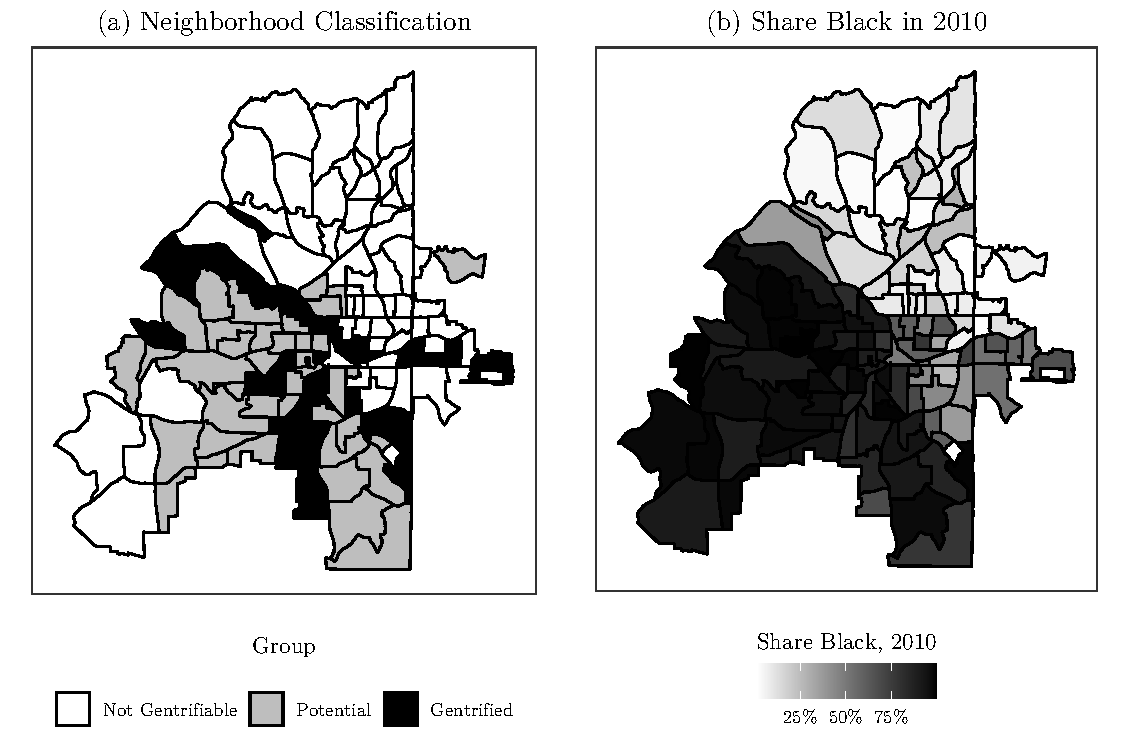
\includegraphics{gentrification_files/figure-latex/maps-1} 

}

\caption{\label{fig:maps}Neighborhood Classification and 2010 Racial Composition}\label{fig:maps}
\end{figure}

In Table \ref{tab:pre-demos}, I present the individual-level characteristics of the voters who fall into each of these three neighborhood types in 2010. Although the age and, to a lesser extent, gender compositions of the neighborhoods are roughly comparable, the similarities end here. While it comes as no surprise that non-gentrifiable neighborhoods in 2010 were whiter, higher-income, and lived in areas with higher home values, the distinctions between the gentrified and gentrifiable neighborhoods bear further scrutiny. While the neighborhoods had similar incomes, the neighborhoods that actually went on to gentrify were considerably less Black than those that did not gentrify. This perhaps points to gentrifier preference for less-Black neighborhoods, a finding corroborated in other scholarship (e.g., \protect\hyperlink{ref-Hwang2014}{Hwang and Sampson 2014}). Of particular note is that gentrified neighborhoods had \emph{lower} rents but \emph{higher} home values in 2010. This could point to the ``rent gap'' identified by \protect\hyperlink{ref-Stein2019}{Stein} (\protect\hyperlink{ref-Stein2019}{2019}) discussed above.

\begin{singlespace}
\begin{table}[!h]

\caption{\label{tab:pre-demo-tab-full}\label{tab:pre-demos} Demographics by Neighborhood Category, 2010}
\centering
\begin{tabular}[t]{llll}
\toprule
Variable & Gentrifiable & Gentrified & Not Gentrifiable\\
\midrule
\% White & 6.1\% & 14.6\% & 59.1\%\\
\% Black & 79.0\% & 69.6\% & 25.2\%\\
\% Male & 44.4\% & 47.8\% & 49.8\%\\
Birth Year & 1966.7 & 1966.6 & 1966.3\\
Median Income & \$16,242.47 & \$17,113.47 & \$46,212.63\\
Median Gross Rent & \$798.99 & \$729.71 & \$1,028.99\\
\% Renters & 60.5\% & 61.3\% & 44.1\%\\
Median Home Value & \$137,374 & \$164,468 & \$388,216\\
N & 90,325 & 49,601 & 163,869\\
\bottomrule
\end{tabular}
\end{table}
\end{singlespace}

\hypertarget{empirical-approach}{%
\subsection{Empirical Approach}\label{empirical-approach}}

To test the turnout effects of exposure to gentrification, I rely on difference-in-differences (DID) models, a common way of establishing causality across the social sciences. In the classical DID set-up, one group of observations receives a ``treatment''---usually exposure to some sort of policy---while another group is not treated. These groups need not be identical prior to the treatment event; instead, DID imposes the assumption that, \emph{in the absence of the treatment}, the outcome variable would have moved in parallel for the two groups. Any observed deviation from these ``parallel trends'' can then be attributed to the treatment. Of course, as Table \ref{tab:pre-demos} makes clear, there are important racial differences between the treatment and control groups. Members of different racial groups might be differentially mobilized over the period and in different elections, leading to violations of the parallel trends assumption that are not attributable to living in a gentrified neighborhood.

One method of improving the plausibility of the parallel trends assumption is to mechanically remove differences between treated and control groups by using matching methodologies to create a subset of control observations that closely mirror the treated voters along a battery of observable characteristics (\protect\hyperlink{ref-Basu2020}{Basu and Small 2020}). While this results in a smaller pool of control observations, it ensures that there are fewer differences between the two groups. I implement this approach in this project, using a genetic matching algorithm (\protect\hyperlink{ref-Sekhon2011}{Sekhon 2011}) to match each treated voter (that is, each voter who lived in 2010 in a neighborhood that would go on to gentrify) to one control voter (someone who lived in 2010 in a gentrifiable neighborhood that \emph{did not} gentrify over the following decade). Voters are matched exactly using their self-reported race (white, Black, or other); their gender; and their turnout in the 2001--2009 local and federal general elections. Voters are also matched (but not exactly) on their year of birth; their registration date; and 2010 neighborhood characteristics (income, rent, share renters, median home value, share white, and share Black).

Because I am also interested in how moving from versus remaining in gentrified neighborhoods shapes participation, I match exactly on whether each voter \emph{did not move}, \emph{moved within Atlanta}, \emph{moved out of Atlanta but in Georgia}, or \emph{dropped out of the dataset}. Thus, I directly compare (for instance) the turnout of voters who moved from gentrified neighborhoods to that of those who moved from gentrifiable neighborhoods. This allows me to sidestep any potential issues arising from differential move rates between these groups. In the Supplementary Information (SI), I show that the results are largely consistent when I use a two-step instrumental variables regression rather than include the outcome residential move measures in the matching procedure.

After constructing my sets of treated and control voters, I run a series of DID / two-way fixed effects (TWFE) OLS models, with fixed effects for year and census tract. Because there is no timing heterogeneity in the treatment (neighborhoods are considered gentrified based on their cumulative change between 2010 and 2020), recent discussions about negative weights and other potential problems with TWFE models do not apply (e.g., \protect\hyperlink{ref-Roth2022}{Roth et al. 2022}).

\hypertarget{residential-moves}{%
\section{Residential Moves}\label{residential-moves}}

Before turning to the turnout analyses, I begin by asking a series of questions central to gentrification studies: are individuals who live in neighborhoods that gentrify more likely to move, or do they remain in place, able to enjoy the potential increase in benefits that attend to a newly-affluent community? And, for those who do leave gentrifying neighborhoods behind, do they leverage some of the increased value in their old community and move to higher-income neighborhoods? Or are they pushed to other low-income neighborhoods?

To untangle these questions, I use a number of multinomial logistic regressions. In each of the models, I limit the pool to registered voters who lived in neighborhoods that were gentrifiable in 2010, testing whether the outcomes for voters who lived in neighborhoods that gentrified (``treated'' voters) differed systematically from those who lived in neighborhoods that did not (``control'' voters). In the first model, presented in Figure \ref{fig:move-multi}, I test whether treated voters were more likely to remain at their 2010 address, move within Atlanta, move outside of Georgia but within Atlanta, or drop out of the administrative records. In the first row, I present the simple means for each group. In the second row of the figure, I include a set of covariates (age; race; gender; registration date, to control for how up-to-date the administrative record is; and neighborhood income, rent, share renters, and home value in 2010). These covariates are held at their means in the plot; the full regression tables can be found in the SI.

\begin{figure}[H]

{\centering 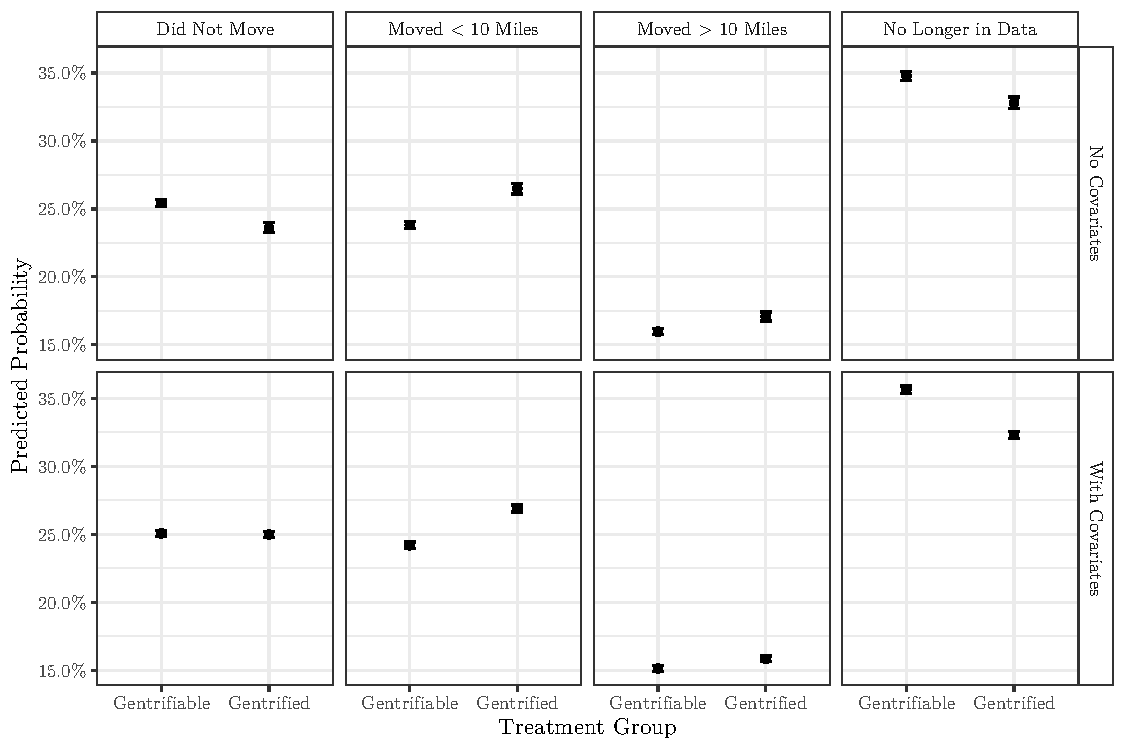
\includegraphics{gentrification_files/figure-latex/move-marg-1} 

}

\caption{\label{fig:move-multi}Predicted Probabilities of Residential Moves}\label{fig:move-marg}
\end{figure}

After controlling for covariates, voters in gentrified neighborhoods were only slightly more likely to move than those in gentrifiable neighborhoods. Conditional on moving, however, their destinations differed in important ways. Voters leaving gentrified neighborhoods were considerably more likely to move within Atlanta; voters leaving gentrifiable neighborhoods, on the other hand, were more likely to drop out of the data entirely, probably indicating that they moved out-of-state. Regardless of the reason for not being observed in the data in 2020, control voters were less likely to be part of the registered electorate in Georgia 10 years later. Only a relatively small share of each group (around 20\%) left Atlanta but remained in Georgia.

Having established that treated voters not substantively more likely to move than untreated voters over the 2010--2020 decade, I now investigate whether voters who lived in gentrified and gentrifiable neighborhoods ended the decade in systematically different types of neighborhoods. In Figure \ref{fig:marg-inc}(A) I plot the predicted median income of the tracts in which the voters lived in 2020, based on their original neighborhood type and whether or not they moved. Figure \ref{fig:marg-inc}(B) plots the 2020 median gross rent of the neighborhoods in which these voters lived at decade's end. I include individual- and neighborhood-level covariates, and robust standard errors are clustered by voters' 2010 tracts. Because we do not know where voters who left the data lived in 2020, these estimates are conditional on still being registered in 2020. The full regression table can be found in the SI.

\begin{figure}[H]

{\centering 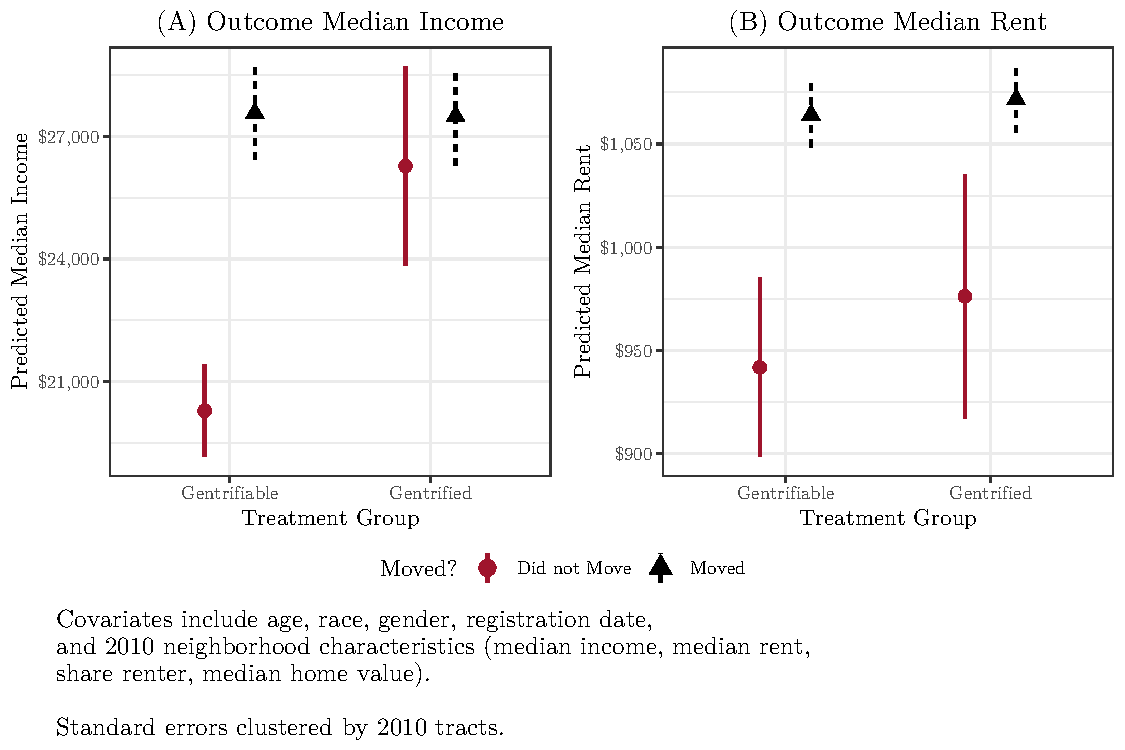
\includegraphics{gentrification_files/figure-latex/move-inc-1} 

}

\caption{\label{fig:marg-inc}Predicted Income Based on Origin Neighborhood Type and Move Status}\label{fig:move-inc}
\end{figure}

Figure \ref{fig:marg-inc}(A) indicates that voters who left gentrifiable neighborhoods ended up in census tracts that differed markedly from their neighborhood of origin: while their original neighborhoods ended the decade with median incomes around \$21,000, those who moved lived in neighborhoods with median incomes closer to \$27,000. By definition, gentrified neighborhoods ended the period with substantially higher incomes than gentrifiable neighborhoods; this is part of the definition of gentrification used here. Of interest, however, is that those who \emph{left} gentrified neighborhoods did not move to neighborhoods with higher incomes than those they left behind, nor than those who left neighborhoods that did not gentrify.

Similarly, Figure \ref{fig:marg-inc}(B) fails to uncover any evidence that movers from different types of original neighborhoods ended up in tracts with systematically different median rents. Movers from both gentrified and gentrifiable neighborhoods ended up in tracts with substantially higher rents than those who remained behind in either type of neighborhood. This is a particularly interesting outcome for individuals who left gentrified neighborhoods: the average mover, it seems, did \emph{not} get pushed to more peripheral neighborhoods where rents were lower than their newly-gentrified origin neighborhoods. Figure \ref{fig:marg-inc} indicates that \emph{movers} as a whole decamped for similar neighborhoods, regardless of the type of neighborhood they left behind.

In sum, voters seem to leave gentrifying neighborhoods behind at slightly higher rates than gentrifiable neighborhoods. Nevertheless, it seems that individuals characteristics associated with moving---and not gentrification---predict the sorts of destination neighborhoods in which movers found themselves at decade's end.

\hypertarget{turnout-analyses}{%
\section{Turnout Analyses}\label{turnout-analyses}}

I now turn to the central question of this project: did the local political participation of voters from gentrified neighborhoods change in marked ways relative to voters from gentrifiable neighborhoods? The previous section tempers our expectations of the politicizing effect of \emph{moving} from a gentrified neighborhood. As that section demonstrated, movers from gentrified and gentrifiable neighborhoods ended the decade in comparable census tracts, at least as measured by income and rent measures. Because the moves did not result in substantially different neighborhood types, and there was relatively little difference in move-rates, it seems less likely that voters leaving behind gentrified neighborhoods would have a markedly different change in their relationship to government as those who left gentrifiable neighborhoods.

By way of reminder, the turnout analyses rely on matched difference-in-difference models. Each voter who in 2010 lived in a tract that would go on to gentrify is matched with one voter in a gentrifiable neighborhood. These are our treatment and control voters. In Figure \ref{fig:local-turnout-plot} I plot the turnout for the treated and selected control voters in odd-numbered years between 2001 and 2021.

\begin{figure}[H]

{\centering 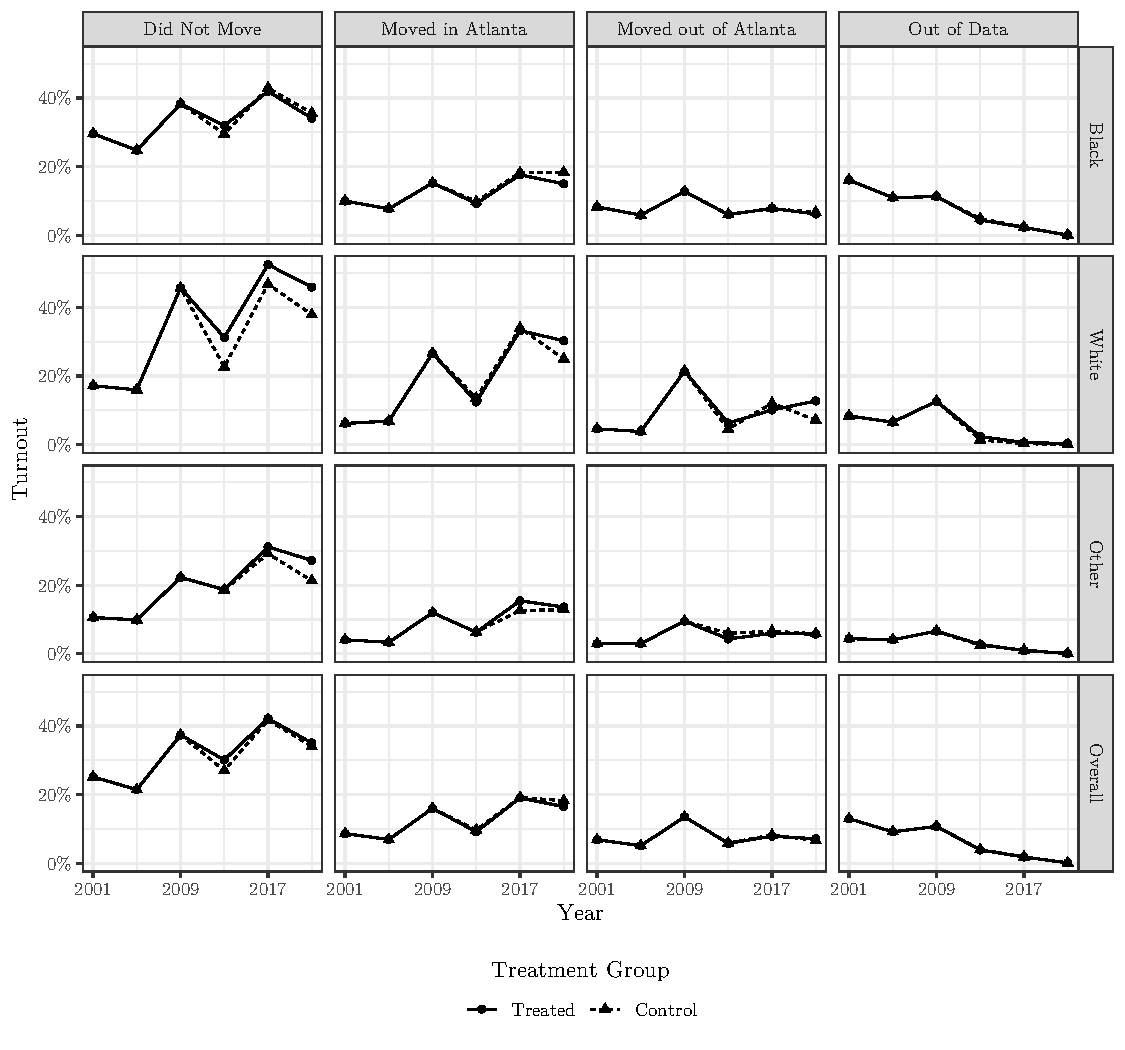
\includegraphics{gentrification_files/figure-latex/to-1-1} 

}

\caption{\label{fig:local-turnout-plot}Turnout in Local Races}\label{fig:to-1}
\end{figure}

Figure \ref{fig:local-turnout-plot} makes immediately clear the absence of large turnout effects pushing in either direction in most cases. Generally speaking, treated Black voters turn out at the same rate in the 2010--2020 period as Black voters who lived in gentrifiable neighborhoods, regardless of whether they moved or not. The same is true of voters who were neither white nor Black. The figure provides visual evidence, however, that white voters who lived in 2010 in neighborhoods that would gentrify turned out at higher rates over the following decade. These plots, however, do not econometrically test the relationships.

To test the statistical significance of these relationships, I use a two-way fixed effects model estimated using ordinary least squares. These models, estimated for each racial group and each move status, include fixed effects for year and 2010 census tract. Robust standard errors are clustered by 2010 census tract, individual voter, and matched set of voters (following the multiway clustering approach of \protect\hyperlink{ref-Cameron2011}{Cameron, Gelbach, and Miller} (\protect\hyperlink{ref-Cameron2011}{2011})). While the full regression tables can be found in the SI, I here present the estimated treatment effect for each group in Figure \ref{fig:local-turnout-ests}. These estimates and confidence intervals are presented from models run with and without the individual-level covariates used in the matching procedure (because of the census tract fixed effects, characteristics that vary at the tract-level drop out of the models).

\begin{figure}[H]

{\centering 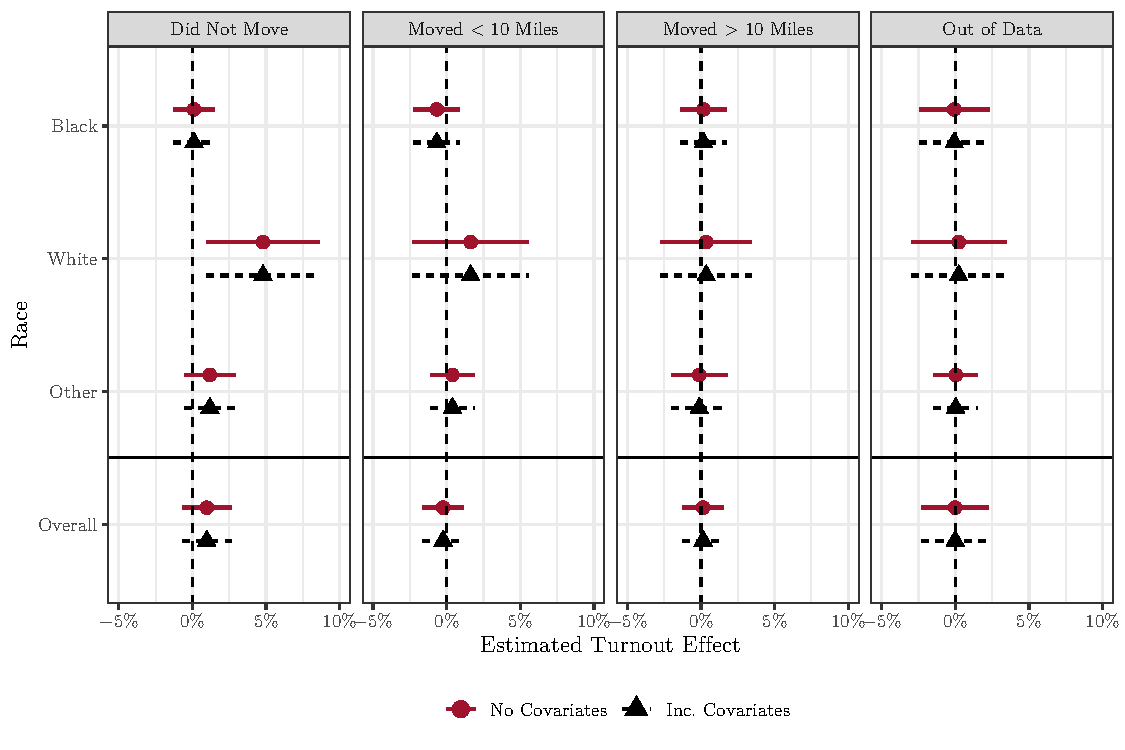
\includegraphics{gentrification_files/figure-latex/to-2-1} 

}

\caption{\label{fig:local-turnout-ests}Estimated Turnout Effects}\label{fig:to-2}
\end{figure}

Figure \ref{fig:local-turnout-ests} provides corroboration for the visual evidence presented in Figure \ref{fig:local-turnout-plot}. The only group for which a statistically significant treatment effect is estimated are white voters who remained behind in gentrified neighborhoods; the post-2010 turnout rate for this group was, on average, about 5 percentage points higher than their matched controls (that is, white individuals who did not move away from gentrifiable neighborhoods).

\hypertarget{discussion-and-conclusion}{%
\section{Discussion and Conclusion}\label{discussion-and-conclusion}}

As detailed in the introduction and theoretical sections of this paper, there is growing evidence that residents of gentrifying neighborhoods understand the state's role in their changing environment better, perhaps, than do many academics. While a handful of qualitative papers document sites of resistance to the neoliberal (municipal) state easing the path of capital and redevelopment in their neighborhoods, few studies have explored the politicizing potentialities of gentrification on neighborhoods as a whole. Considering the volume of work on the effects of gentrification on schooling, employment, health, and other social indicators, the literature's silence on this question is puzzling.

This study indicates that---at least in the case of Atlanta in the 2010s---the \emph{average} Black resident of a gentrifying neighborhood is neither more nor less likely to participate in local electoral politics than residents of similar neighborhoods that do not gentrify. To be sure, this does not discount the work being done by activists such as Bertha Darden and members of her community, who have applied intense political pressure. Indeed, as noted above, Mayor Dickens made housing affordability and protections against gentrification central to his 2021 campaign. Although I do not find evidence that gentrification increased the turnout of Black residents in local contests, this should not be interpreted to mean that (Black) Atlantans have not successfully politicized the issue.

How, then, do we make sense of these results? Given plentiful evidence that electoral candidates in the city feel the need to speak explicitly about housing and gentrification, how do we make sense of the null findings with respect to turnout? There are a number of potential explanations that scholars should take up and investigate, in the context of Atlanta and elsewhere. It is also worth noting that the results presented here represent \emph{average} treatment effects; I am unable to identify whether there are small effects across-the-board, or if gentrification is \emph{mobilizing} for some residents even as it \emph{demobilizes} others, leading to effects that cancel one another.

The first possibility turns on the identification mechanism I use in this study. Although census tracts are intended to be ``as homogeneous as possible with respect to population characteristics, economic status, and living condition,''\footnote{See \url{https://www2.census.gov/geo/pdfs/reference/GARM/Ch10GARM.pdf}.} these borders may not be as salient for the lived political realities of Black residents of Atlanta. In other words, although one voter may live in a \emph{gentrified} tract while another lived in a \emph{gentrifiable} tract---the heart of my binary treatment assignment---, it seems possible that the ways in which individuals make sense of their neighborhoods and communities are more complex. This might be especially true if treated and control voters were drawn from abutting or geographically-proximate neighborhoods. Voters in gentrifiable tracts might still see an influx of newcomers in their grocery stores and on their bus routes, even if their particular tract's median did not increase enough to qualify as gentrifying.

Voters might also not have distinguished between hyperlocal, tract-level changes and changes throughout the city. While rents increased by more than 50\% in gentrified tracts, they also increased meaningfully in gentrifiable tracts (by 20\%). Similarly, even gentrified tracts remained overwhelmingly Black by decade's end, as were gentrifiable neighborhoods (see Figure \ref{fig:local-race}. Nevertheless, the plausibility that residents of gentrifiable neighborhoods perceived as much change---and were thus equally politicized as those in gentrified neighborhoods---is strained. Not only did rents increase far more in gentrified neighborhoods; incomes in these neighborhoods also increased far more, by 60\% and 12\%, respectively. Moreover, as Figure \ref{fig:local-race} indicates, the 2010--2020 decade saw markedly distinct racial patterns in the two types of neighborhoods. Although both gentrified and gentrifiable neighborhoods saw similar trends in the Black share of the population prior to the decade under study, the next decade looked different. While gentrifiable neighborhoods re-segregated to a certain extent and became more-Black, the Black share of the population in gentrified tracts continued to erode. Thus, although citywide narratives about gentrification might have had effects throughout the city, gentrified neighborhoods were in fact subject to substantially distinct sociodemographic conditions over the period relative to gentrifiable ones.

\begin{figure}[H]

{\centering 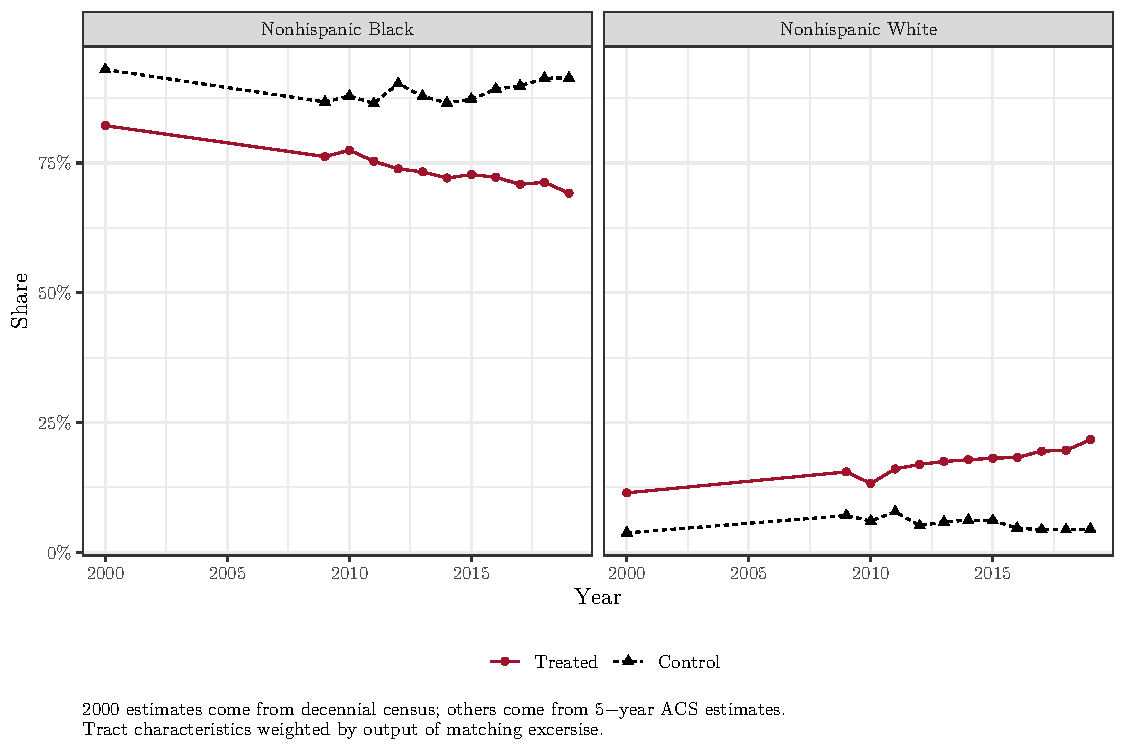
\includegraphics{gentrification_files/figure-latex/race-time-1} 

}

\caption{\label{fig:local-race}Racial Composition, Treated and Control Tract}\label{fig:race-time}
\end{figure}

Figure \ref{fig:local-race} also points us back to the only group for which I uncover a statistically significant treatment effect: white voters who lived in 2010 in tracts that went on to gentrify. Somewhat surprisingly, the experience of living in a neighborhood that gentrified substantially increased the turnout of these voters. While this project did not theoretically situate any expected politicization for this group---aside from an expectation that gentrification would be \emph{more likely} to politicize longer-term Black residents---there is clearly some sort of political socialization occurring in this population. Increasing numbers of residents who ``look like them'' (the white share of the gentrified tracts increased by 40\%) could have increased political efficacy; political campaigns may have changed tactics to center the needs of this growing population, thereby mobilizing; or something else entirely may be at work. Both by virtue of population growth and increasing participation, the white share of the electorate is increasing substantially in these neighborhoods. Future scholarship should investigate the consequences of such changes, and assess whether the newcomers exhibit marked differences in electoral preferences and thus present a political threat to the established community.

Another potential explanation lies in Figure \ref{fig:marg-inc}. Although much of the public discussion around gentrification returns to concerns about residents being pushed out of their neighborhoods, the results from Atlanta paint a more complicated picture. If displacement were driving neighborhood turnover, we would expect to see individuals who leave gentrified neighborhoods to relocate to areas that ended the decade with lower rents than their neighborhood of origin; in fact, I find the exact opposite here. Although gentrified neighborhoods did---by definition---experience above-average growth in housing costs, Atlantas leaving gentrified neighborhoods relocated to tracts with \emph{even higher} housing costs. In other words, the theorized ``threat'' of gentrification did not necessarily materialize as expected: most residents of gentrified neighborhoods either did not move, or relocated to higher rent / income neighborhoods. Put differently, the average resident neither experienced being pushed out of their home, nor watched this happen to a neighborhood. It bears repeating that these models measure the \emph{average} outcome, which is certainly not to say that no residents were displaced into lower-income neighborhoods. Future work should investigate whether heterogeneity in why individuals leave their neighborhoods structures political identify and participation.

The translation of state-sponsored action into mass political action is a slow process; this is undoubtedly especially true of processes like gentrification and neighborhood change, which occur block-by-block and are distinguished by a mix of \emph{positive} investments in public goods even as long-term residents face rising unaffordability. It is perhaps thus unsurprising that, despite extensive scholarship documenting the mobilization of \emph{some} residents in community organizations to combat gentrification, I uncover no evidence that the turnout of the average Black resident changes thanks to seeing their neighborhood gentrify, whether they remained in their original neighborhood or not. I do find that individuals who leave gentrifying neighborhoods relocate to higher income neighborhoods, but this does not appear to impact their electoral participation. Scholars and activists should continue to investigate these relationships, asking whether, when, and how the state-sanctioned processes of gentrification can be contested at the ballot box.

\newpage

\hypertarget{references}{%
\section*{References}\label{references}}
\addcontentsline{toc}{section}{References}

\hypertarget{refs}{}
\begin{CSLReferences}{1}{0}
\leavevmode\hypertarget{ref-Almeida2018}{}%
Almeida, Paul D. 2018. {``The {Role} of {Threat} in {Collective Action}.''} In \emph{The {Wiley Blackwell Companion} to {Social Movements}}, edited by David A. Snow, Sarah A. Soule, Hanspeter Kriesi, and Holly J. McCammon, 43--62. {John Wiley \& Sons, Ltd}. \url{https://doi.org/10.1002/9781119168577.ch2}.

\leavevmode\hypertarget{ref-Amy2021}{}%
Amy, Jeff. 2021. {``Georgia Officials Seek to Remove 102,000 Voters from Rolls.''} \emph{AP News: GA State Wire}, June 18, 2021. \url{https://apnews.com/article/ga-state-wire-georgia-election-2020-voter-registration-business-a916e90db938aa60a4eff3d00d391006}.

\leavevmode\hypertarget{ref-Ashly2020}{}%
Ashly, Jaclynn. 2020. {``The {Black} Residents Fighting {Atlanta} to Stay in Their Homes.''} \emph{Al Jazeera}, November 30, 2020. \url{https://www.aljazeera.com/features/2020/11/30/atlanta-gentrification}.

\leavevmode\hypertarget{ref-Barrie2021}{}%
Barrie, Christopher. 2021. {``Political Sociology in a Time of Protest.''} \emph{Current Sociology}, June, 00113921211024692. \url{https://doi.org/10.1177/00113921211024692}.

\leavevmode\hypertarget{ref-Basu2020}{}%
Basu, Pallavi, and Dylan S. Small. 2020. {``Constructing a {More Closely Matched Control Group} in a {Difference-in-Differences Analysis}: {Its Effect} on {History Interacting} with {Group Bias}.''} \emph{Observational Studies} 6 (1): 103--30. \url{https://doi.org/10.1353/obs.2020.0011}.

\leavevmode\hypertarget{ref-Betancur2002}{}%
Betancur, John. 2002. {``The {Politics} of {Gentrification}: {The Case} of {West Town} in {Chicago}.''} \emph{Urban Affairs Review} 37 (6): 780--814. \url{https://doi.org/10.1177/107874037006002}.

\leavevmode\hypertarget{ref-Betancur2011}{}%
---------. 2011. {``Gentrification and {Community Fabric} in {Chicago}.''} \emph{Urban Studies} 48 (2): 383--406. \url{https://doi.org/10.1177/0042098009360680}.

\leavevmode\hypertarget{ref-Birch2009}{}%
Birch, Eugénie L. 2009. {``Downtown in the {`{New American City}'}.''} \emph{The ANNALS of the American Academy of Political and Social Science} 626 (1): 134--53. \url{https://doi.org/10.1177/0002716209344169}.

\leavevmode\hypertarget{ref-Cameron2011}{}%
Cameron, A. Colin, Jonah B. Gelbach, and Douglas L. Miller. 2011. {``Robust {Inference With Multiway Clustering}.''} \emph{Journal of Business \& Economic Statistics} 29 (2): 238--49. \url{http://www.jstor.org/stable/25800796}.

\leavevmode\hypertarget{ref-Capelouto2021}{}%
Capelouto, J. D., Emily Merwin DiRico, and John Perry. 2021. {``As {Atlanta}'s Population Changes, so Does the Race for Mayor.''} \emph{The Atlanta Journal-Constitution: Local News}, August 26, 2021.

\leavevmode\hypertarget{ref-Dastrup2016}{}%
Dastrup, Samuel, and Ingrid Gould Ellen. 2016. {``Linking {Residents} to {Opportunity}: {Gentrification} and {Public Housing}.''} \emph{Cityscape} 18 (3): 87--108. \url{http://www.jstor.org/stable/26328274}.

\leavevmode\hypertarget{ref-Deere2020}{}%
Deere, Stephen. 2020. {``Group Says {Atlanta Mayor Bottoms} Not Fighting Gentrification.''} \emph{The Atlanta Journal-Constitution: Politics}, March 4, 2020.

\leavevmode\hypertarget{ref-Dragan2020}{}%
Dragan, Kacie, Ingrid Gould Ellen, and Sherry Glied. 2020. {``Does Gentrification Displace Poor Children and Their Families? {New} Evidence from Medicaid Data in {New York City}.''} \emph{Regional Science and Urban Economics} 83 (July): 103481. \url{https://doi.org/10.1016/j.regsciurbeco.2019.103481}.

\leavevmode\hypertarget{ref-Easton2020}{}%
Easton, Sue, Loretta Lees, Phil Hubbard, and Nicholas Tate. 2020. {``Measuring and Mapping Displacement: {The} Problem of Quantification in the Battle Against Gentrification.''} \emph{Urban Studies} 57 (2): 286--306. \url{https://doi.org/10.1177/0042098019851953}.

\leavevmode\hypertarget{ref-Edelmann2020}{}%
Edelmann, Achim, Tom Wolff, Danielle Montagne, and Christopher A. Bail. 2020. {``Computational {Social Science} and {Sociology}.''} \emph{Annual Review of Sociology} 46 (1): 61--81. \url{https://doi.org/10.1146/annurev-soc-121919-054621}.

\leavevmode\hypertarget{ref-Freeman2015}{}%
Freeman, Lance, and Tiancheng Cai. 2015. {``White {Entry} into {Black Neighborhoods}: {Advent} of a {New Era}?''} \emph{The Annals of the American Academy of Political and Social Science} 660: 302--18. \url{http://www.jstor.org/stable/24541839}.

\leavevmode\hypertarget{ref-Gerber2008}{}%
Gerber, Alan S., Donald P. Green, and Christopher W. Larimer. 2008. {``Social {Pressure} and {Voter Turnout}: {Evidence} from a {Large-Scale Field Experiment}.''} \emph{American Political Science Review} 102 (1): 33--48. \url{https://doi.org/10.1017/S000305540808009X}.

\leavevmode\hypertarget{ref-Haag2019}{}%
Haag, Matthew. 2019. {``It's {Manhattan}'s {Last Affordable Neighborhood}. {But} for {How Long}?''} \emph{The New York Times: New York}, September 27, 2019. \url{https://www.nytimes.com/2019/09/27/nyregion/its-manhattans-last-affordable-neighborhood-but-for-how-long.html}.

\leavevmode\hypertarget{ref-Habersham2019}{}%
Habersham, Raisa. 2019. {``Some {Spelman} Students Upset {Atlanta} Mayor Is Commencement Speaker.''} \emph{The Atlanta Journal-Constitution: Intown Atlanta}, April 24, 2019.

\leavevmode\hypertarget{ref-Hajnal2009}{}%
Hajnal, Zoltan. 2009. \emph{America's Uneven Democracy: Race, Turnout, and Representation in City Politics}. {Cambridge ; New York}: {Cambridge University Press}.

\leavevmode\hypertarget{ref-Hartman2002}{}%
Hartman, Chester W. 2002. \emph{Between Eminence and Notoriety: Four Decades of Radical Urban Planning}. {New Brunswick, N.J}: {Center for Urban Policy Research}.

\leavevmode\hypertarget{ref-Holmes2020}{}%
Holmes, Kristin E. 2020. {``Religious Agency in the Dynamics of Gentrification: {Moving} in, Moving Out, and Staying Put in {Philadelphia}.''} In \emph{The {Routledge Handbook} of {Religion} and {Cities}}. {Routledge}.

\leavevmode\hypertarget{ref-Huynh2021}{}%
Huynh, Anjali, and Ben Brasch. 2021. {``Atlanta Voters Hope for More Focus on Affordable Housing as Runoff Nears.''} \emph{The Atlanta Journal-Constitution: Local News}, November 13, 2021.

\leavevmode\hypertarget{ref-Hwang2020}{}%
Hwang, Jackelyn, and Lei Ding. 2020. {``Unequal {Displacement}: {Gentrification}, {Racial Stratification}, and {Residential Destinations} in {Philadelphia}.''} \emph{American Journal of Sociology} 126 (2): 354--406. \url{https://doi.org/10.1086/711015}.

\leavevmode\hypertarget{ref-Hwang2014}{}%
Hwang, Jackelyn, and Robert J. Sampson. 2014. {``Divergent {Pathways} of {Gentrification}: {Racial Inequality} and the {Social Order} of {Renewal} in {Chicago Neighborhoods}.''} \emph{American Sociological Review} 79 (4): 726--51. \url{https://doi.org/10.1177/0003122414535774}.

\leavevmode\hypertarget{ref-Hyra2015}{}%
Hyra, Derek. 2015. {``The Back-to-the-City Movement: {Neighbourhood} Redevelopment and Processes of Political and Cultural Displacement.''} \emph{Urban Studies} 52 (10): 1753--73. \url{https://doi.org/10.1177/0042098014539403}.

\leavevmode\hypertarget{ref-Immergluck2018}{}%
Immergluck, Dan, and Tharunya Balan. 2018. {``Sustainable for Whom? {Green} Urban Development, Environmental Gentrification, and the {Atlanta Beltline}.''} \emph{Urban Geography} 39 (4): 546--62. \url{https://doi.org/10.1080/02723638.2017.1360041}.

\leavevmode\hypertarget{ref-Jackson1985}{}%
Jackson, Kenneth T. 1985. \emph{Crabgrass Frontier: The Suburbanization of the {United States}}. {New York}: {Oxford University Press}.

\leavevmode\hypertarget{ref-Kauffman2018}{}%
Kauffman, Johnny. 2018. {``6 {Takeaways From Georgia}'s '{Use It Or Lose It}' {Voter Purge Investigation}.''} \emph{NPR: National}, October 22, 2018. \url{https://www.npr.org/2018/10/22/659591998/6-takeaways-from-georgias-use-it-or-lose-it-voter-purge-investigation}.

\leavevmode\hypertarget{ref-Keels2013}{}%
Keels, Micere, Julia Burdick--Will, and Sara Keene. 2013. {``The {Effects} of {Gentrification} on {Neighborhood Public Schools}.''} \emph{City \& Community} 12 (3): 238--59. \url{https://doi.org/10.1111/cico.12027}.

\leavevmode\hypertarget{ref-Knotts2006}{}%
Knotts, H. Gibbs, and Moshe Haspel. 2006. {``The {Impact} of {Gentrification} on {Voter Turnout}.''} \emph{Social Science Quarterly} 87 (1): 110--21. \url{http://www.jstor.org/stable/42956112}.

\leavevmode\hypertarget{ref-Lartey2018}{}%
Lartey, Jamiles. 2018. {``Nowhere for People to Go: Who Will Survive the Gentrification of {Atlanta}?''} \emph{The Guardian: Cities}, October 23, 2018. \url{http://www.theguardian.com/cities/2018/oct/23/nowhere-for-people-to-go-who-will-survive-the-gentrification-of-atlanta}.

\leavevmode\hypertarget{ref-Latimore2020}{}%
Latimore, Marshall A. 2020. {``Mayor {Keisha Lance Bottoms} Creates Anti-Displacement Tax Fund to Strengthen Homeownership for Legacy Residents \textbar{} {The Atlanta Voice}.''} \emph{The Atlanta Voice}, October 20, 2020. \url{https://www.theatlantavoice.com/articles/mayor-keisha-lance-bottoms-creates-anti-displacement-tax-fund-to-strengthen-homeownership-for-legacy-residents/}.

\leavevmode\hypertarget{ref-Lees2018}{}%
Lees, Loretta, Sandra Annunziata, and Clara Rivas-Alonso. 2018. {``Resisting {Planetary Gentrification}: {The Value} of {Survivability} in the {Fight} to {Stay Put}.''} \emph{Annals of the American Association of Geographers} 108 (2): 346--55. \url{https://doi.org/10.1080/24694452.2017.1365587}.

\leavevmode\hypertarget{ref-Lefebvre1968}{}%
Lefebvre, Henri. 1968. \emph{Le {Droit} à La {Ville}}. {Paris}: {Anthropos}.

\leavevmode\hypertarget{ref-Levine2018}{}%
Levine, Jeremy R., Theodore S. Leenman, Carl Gershenson, and David M. Hureau. 2018. {``Political {Places}: {Neighborhood Social Organization} and the {Ecology} of {Political Behaviors}.''} \emph{Social Science Quarterly} 99 (1): 201--15. \url{https://doi.org/10.1111/ssqu.12352}.

\leavevmode\hypertarget{ref-Martin2007a}{}%
Martin, Leslie. 2007. {``Fighting for {Control}: {Political Displacement} in {Atlanta}'s {Gentrifying Neighborhoods}.''} \emph{Urban Affairs Review} 42 (5): 603--28. \url{https://doi.org/10.1177/1078087406296604}.

\leavevmode\hypertarget{ref-Massey2003}{}%
Massey, Douglas S., and Nancy A. Denton. 2003. \emph{American Apartheid: Segregation and the Making of the Underclass}. 10. print. {Cambridge, Mass.}: {Harvard Univ. Press}.

\leavevmode\hypertarget{ref-McCaffrey2021}{}%
McCaffrey, Shannon. 2021. {``A Long Eviction Fight in {Peoplestown} Reverberates in {Atlanta} Mayor's Race.''} \emph{Atlanta Magazine}, November 23, 2021. \url{https://www.atlantamagazine.com/news-culture-articles/a-long-eviction-fight-in-peoplestown-reverberates-in-atlanta-mayors-race/}.

\leavevmode\hypertarget{ref-Meltzer2017}{}%
Meltzer, Rachel, and Pooya Ghorbani. 2017. {``Does Gentrification Increase Employment Opportunities in Low-Income Neighborhoods?''} \emph{Regional Science and Urban Economics} 66 (September): 52--73. \url{https://doi.org/10.1016/j.regsciurbeco.2017.06.002}.

\leavevmode\hypertarget{ref-Morris2019a}{}%
Morris, Kevin, and Peter Dunphy. 2019. {``{AVR Impact} on {State Voter Registration}.''} {Brennan Center for Justice}. \url{https://www.brennancenter.org/our-work/research-reports/avr-impact-state-voter-registration}.

\leavevmode\hypertarget{ref-Newman2016}{}%
Newman, Benjamin J., Yamil Velez, and Shanna Pearson-Merkowitz. 2016. {``Diversity of a {Different Kind}: {Gentrification} and {Its Impact} on {Social Capital} and {Political Participation} in {Black Communities}.''} \emph{Journal of Race, Ethnicity, and Politics} 1 (2): 316--47. \url{https://doi.org/10.1017/rep.2016.8}.

\leavevmode\hypertarget{ref-Niesse2021a}{}%
Niesse, Mark. 2021. {``Almost All Eligible {Georgians} Are Registered to Vote, Data Show.''} \emph{The Atlanta Journal-Constitution: Politics}, July 19, 2021.

\leavevmode\hypertarget{ref-Papachristos2011}{}%
Papachristos, Andrew V., Chris M. Smith, Mary L. Scherer, and Melissa A. Fugiero. 2011. {``More {Coffee}, {Less Crime}? {The Relationship} Between {Gentrification} and {Neighborhood Crime Rates} in {Chicago}, 1991 to 2005.''} \emph{City \& Community} 10 (3): 215--40. \url{https://doi.org/10.1111/j.1540-6040.2011.01371.x}.

\leavevmode\hypertarget{ref-Phillips-Fein2017}{}%
Phillips-Fein, Kim. 2017. \emph{Fear City: {New York}'s Fiscal Crisis and the Rise of Austerity Politics}. First edition. {New York}: {Metropolitan Books}.

\leavevmode\hypertarget{ref-Piven1979}{}%
Piven, Frances Fox, and Richard A. Cloward. 1979. \emph{Poor People's Movements: Why They Succeed, How They Fail}. {New York}: {Vintage books}.

\leavevmode\hypertarget{ref-Reese2011}{}%
Reese, Ellen. 2011. \emph{They {Say Cutback}, {We Say Fight Back}!: {Welfare Activism} in an {Era} of {Retrenchment}}. {New York, UNITED STATES}: {Russell Sage Foundation}. \url{http://ebookcentral.proquest.com/lib/nyulibrary-ebooks/detail.action?docID=4386937}.

\leavevmode\hypertarget{ref-Riker1968}{}%
Riker, William H., and Peter C. Ordeshook. 1968. {``A {Theory} of the {Calculus} of {Voting}.''} \emph{The American Political Science Review} 62 (1): 25--42. \url{https://doi.org/10.2307/1953324}.

\leavevmode\hypertarget{ref-Roth2022}{}%
Roth, Jonathan, Pedro H. C. Sant'Anna, Alyssa Bilinski, and John Poe. 2022. {``What's {Trending} in {Difference-in-Differences}? {A Synthesis} of the {Recent Econometrics Literature}.''} \url{http://arxiv.org/abs/2201.01194}.

\leavevmode\hypertarget{ref-Rothstein2017}{}%
Rothstein, Richard. 2017. \emph{The Color of Law: A Forgotten History of How Our Government Segregated {America}}. First edition. {New York ; London}: {Liveright Publishing Corporation, a division of W. W. Norton \& Company}.

\leavevmode\hypertarget{ref-Savage2007}{}%
Savage, Mike, and Roger Burrows. 2007. {``The {Coming Crisis} of {Empirical Sociology}.''} \emph{Sociology} 41 (5): 885--99. \url{https://doi.org/10.1177/0038038507080443}.

\leavevmode\hypertarget{ref-Schlozman1979}{}%
Schlozman, Kay Kehman, and Sidney Verba. 1979. \emph{Injury to {Insult}: {Unemployment}, {Class}, and {Political Response}}. {Harvard University Press}. \url{http://books.google.com?id=m6XTdRlx3Q8C}.

\leavevmode\hypertarget{ref-Sekhon2011}{}%
Sekhon, Jasjeet S. 2011. {``Multivariate and {Propensity Score Matching Software} with {Automated Balance Optimization}: {The Matching} Package for {R}.''} \emph{Journal of Statistical Software} 42 (7): 1--52. \url{https://doi.org/10.18637/jss.v042.i07}.

\leavevmode\hypertarget{ref-Smith2002}{}%
Smith, Neil. 2002. {``New {Globalism}, {New Urbanism}: {Gentrification} as {Global Urban Strategy}.''} \emph{Antipode} 34 (3): 427--50. \url{https://doi.org/10.1111/1467-8330.00249}.

\leavevmode\hypertarget{ref-Stein2019}{}%
Stein, Samuel. 2019. \emph{Capital City: Gentrification and the Real Estate State}. Jacobin Series. {London ; Brooklyn, NY}: {Verso}.

\leavevmode\hypertarget{ref-vanStekelenburg2013}{}%
Stekelenburg, Jacquelien van, and Bert Klandermans. 2013. {``The Social Psychology of Protest.''} \emph{Current Sociology} 61 (5-6): 886--905. \url{https://doi.org/10.1177/0011392113479314}.

\leavevmode\hypertarget{ref-Sugrue1998}{}%
Sugrue, Thomas J. 1998. \emph{The Origins of the Urban Crisis: Race and Inequality in Postwar {Detroit}}. 1st paperback ed. Princeton Studies in {American} Politics. {Princeton, N.J}: {Princeton University Press}.

\leavevmode\hypertarget{ref-TamCho2006a}{}%
Tam Cho, Wendy K., James G. Gimpel, and Tony Wu. 2006. {``Clarifying the {Role} of {SES} in {Political Participation}: {Policy Threat} and {Arab American Mobilization}.''} \emph{Journal of Politics} 68 (4): 977--91. \url{https://doi.org/10.1111/j.1468-2508.2006.00482.x}.

\leavevmode\hypertarget{ref-Taylor2019}{}%
Taylor, Keeanga-Yamahtta. 2019. \emph{Race for Profit: How Banks and the Real Estate Industry Undermined Black Homeownership}. Justice, Power, and Politics. {Chapel Hill}: {The University of North Carolina Press}.

\leavevmode\hypertarget{ref-Theodore2020}{}%
Theodore, Nik. 2020. {``Governing Through Austerity: ({Il})logics of Neoliberal Urbanism After the Global Financial Crisis.''} \emph{Journal of Urban Affairs} 42 (1): 1--17. \url{https://doi.org/10.1080/07352166.2019.1623683}.

\leavevmode\hypertarget{ref-Thompson2020}{}%
Thompson, Laura. 2020. {``The Cop Who Quit Instead of Helping to Gentrify {Atlanta}.''} \emph{Mother Jones}, September 14, 2020. \url{https://www.motherjones.com/crime-justice/2020/09/the-cop-who-quit-instead-of-helping-to-gentrify-atlanta/}.

\leavevmode\hypertarget{ref-Thorpe2021}{}%
Thorpe, Amelia. 2021. {``Regulatory Gentrification: {Documents}, Displacement and the Loss of Low-Income Housing.''} \emph{Urban Studies} 58 (13): 2623--39. \url{https://doi.org/10.1177/0042098020960569}.

\leavevmode\hypertarget{ref-Towler2018}{}%
Towler, Christopher C., and Christopher S. Parker. 2018. {``Between {Anger} and {Engagement}: {Donald Trump} and {Black America}.''} \emph{Journal of Race, Ethnicity, and Politics} 3 (1): 219--53. \url{https://doi.org/10.1017/rep.2017.38}.

\leavevmode\hypertarget{ref-Verba1995}{}%
Verba, Sidney, Kay Lehman Schlozman, and Henry E. Brady. 1995. \emph{Voice and {Equality}: {Civic Voluntarism} in {American Politics}}. {Harvard University Press}. \url{http://books.google.com?id=RUkvEAAAQBAJ}.

\leavevmode\hypertarget{ref-Webber2009}{}%
Webber, Richard. 2009. {``Response to {`{The Coming Crisis} of {Empirical Sociology}'}: {An Outline} of the {Research Potential} of {Administrative} and {Transactional Data}.''} \emph{Sociology} 43 (1): 169--78. \url{https://doi.org/10.1177/0038038508099104}.

\leavevmode\hypertarget{ref-Weber2002}{}%
Weber, Rachel. 2002. {``Extracting {Value} from the {City}: {Neoliberalism} and {Urban Redevelopment}.''} \emph{Antipode} 34 (3): 519--40. \url{https://doi.org/10.1111/1467-8330.00253}.

\leavevmode\hypertarget{ref-White2016}{}%
White, Ariel. 2016. {``When {Threat Mobilizes}: {Immigration Enforcement} and {Latino Voter Turnout}.''} \emph{Political Behavior} 38 (2): 355--82. \url{https://doi.org/10.1007/s11109-015-9317-5}.

\leavevmode\hypertarget{ref-Zepeda-Millan2016}{}%
Zepeda-Millán, Chris. 2016. {``Weapons of the ({Not So}) {Weak}: {Immigrant Mass Mobilization} in the {US South}.''} \emph{Critical Sociology} 42 (2): 269--87. \url{https://doi.org/10.1177/0896920514527846}.

\leavevmode\hypertarget{ref-Zuk2015}{}%
Zuk, Miriam, Ariel Bierbaum, Karolina Gorska, Anastasia Loukaitou-Sideris, Paul Ong, Trevor Thomas, and Karen Chapple. 2015. \emph{Gentrification, {Displacement} and the {Role} of {Public Investment}: {A Literature Review}}. {Federal Reserve Bank of San Francisco}. \url{https://doi.org/10.13140/RG.2.2.12408.60168}.

\leavevmode\hypertarget{ref-Zukin2009}{}%
Zukin, Sharon, Valerie Trujillo, Peter Frase, Danielle Jackson, Tim Recuber, and Abraham Walker. 2009. {``New {Retail Capital} and {Neighborhood Change}: {Boutiques} and {Gentrification} in {New York City}.''} \emph{City \& Community} 8 (1): 47--64. \url{https://doi.org/10.1111/j.1540-6040.2009.01269.x}.

\end{CSLReferences}

\end{document}
